\documentclass{article}
\usepackage{amsmath}
\usepackage{listings}
\usepackage[utf8]{inputenc}
\usepackage{graphicx}

\graphicspath{ {../output/} }

\lstset{
	basicstyle=\footnotesize,
	numbers=left,
	tabsize=3,
	title=\lstname,
	breaklines=true
}

\addtolength{\oddsidemargin}{-.875in}
\addtolength{\evensidemargin}{-.875in}
\addtolength{\textwidth}{1.75in}

\addtolength{\topmargin}{-.875in}
\addtolength{\textheight}{1.75in}

\title{Lernverfahren autonomer Roboter - Übung 3}
\author{Tobias Hahn\\ 3073375}	
	
\begin{document}
\maketitle
\newpage
\section{Übung 3}
\subsection{Performance metrics}
\subsubsection{}
In order to calculate all these scores, we first need to calculate some basis data from our results. Namely we need to count the amount of true and false positives and negatives.
\paragraph{}
\begin{tabular}{|l|l|l|}
	\hline
	Type & Positives & Negatives \\\hline
	True & 5 & 81 \\\hline
	False & 5 & 9 \\\hline
\end{tabular}

\subsubsection{Accuracy}
The Accuracy unseres Klassifizierers therefore is:
\[
	Accuracy = \frac{TP + TN}{P + N} = \frac{5 + 81}{10 + 90} = frac{86}{100} = 0.86
\]

\subsubsection{Specificity}
The Specificity (true negative rate) is:
\[
	Specificity = \frac{TN}{N} = \frac{81}{90} = 0.9
\]

\subsubsection{F-measure}
The F-measure is:
\[
	F-measure = \frac{2 * TP}{2 * TP + FP + FN} = \frac{2 * 5}{2 * 5 + 5 + 9} = \frac{10}{24} \approx 0.417
\]

\subsubsection{Normalized mutual information}
The Normalized mutual information is:
\begin{align*}
	&\textrm{Normalized mutual information} = \frac{H(T) - H(T|Y)}{H(T)}\\
	&= \frac{ -(0.1 * \log_2 0.1 + 0.9 * \log_2 0.9) - (0.81 * \log {\frac{0.9}{0.81}} + 0.05 * \log {\frac{0.1}{0.05}} + 0.09 * \log {\frac{0.9}{0.09}} + 0.05 * \log{\frac{0.1}{0.05}})}{-(0.1 * \log_2 0.1 + 0.9 * \log_2 0.9)}\\
	&\approx \frac{0.107}{0.469} \approx 0.228
\end{align*}

\subsubsection{Matthew's correlation coefficient}
Matthew's correlation coefficient is:
\begin{align*}
	&\textrm{Matthew's correlation coefficient} = \frac{TP * TN + FP * FN}{\sqrt{(TP + FP)(TP + FN)(TN + FP)(TN + FN)}}\\
	&= \frac{5 * 81 + 5 * 9}{\sqrt{25 * 14 * 86 * 90}} = \frac{450}{\sqrt{2709000}} \approx 0.273 
\end{align*}

\subsubsection{Merrit of Accuracy}
Accuracy is not a good measure of the merrit of our classifier in this case. This is because the magnitude of both classes is very unequal: While there are 90 examples of negative values, there are only 10 positive examples. Accuracy only measures the amount of times our classifier gets it right, but in our case we are more interested in the ability of the classifier to distinguish positive from negative examples. For example, a classifier that would predict false very time would have an accuracy of 0.9 here, although next to useless for classification.

\subsection{ROC Curve and AUC Score}
The ROC curve is calculated by taking the unique prediciton values from our classifier and calculating the respective rates (false positive rate and true positive rate) for this threshold. Then we plot all the points on a curve, and therefore get a graph showing us how good our classifier does for a specified threshold.

\begin{figure}[h]
    \centering
    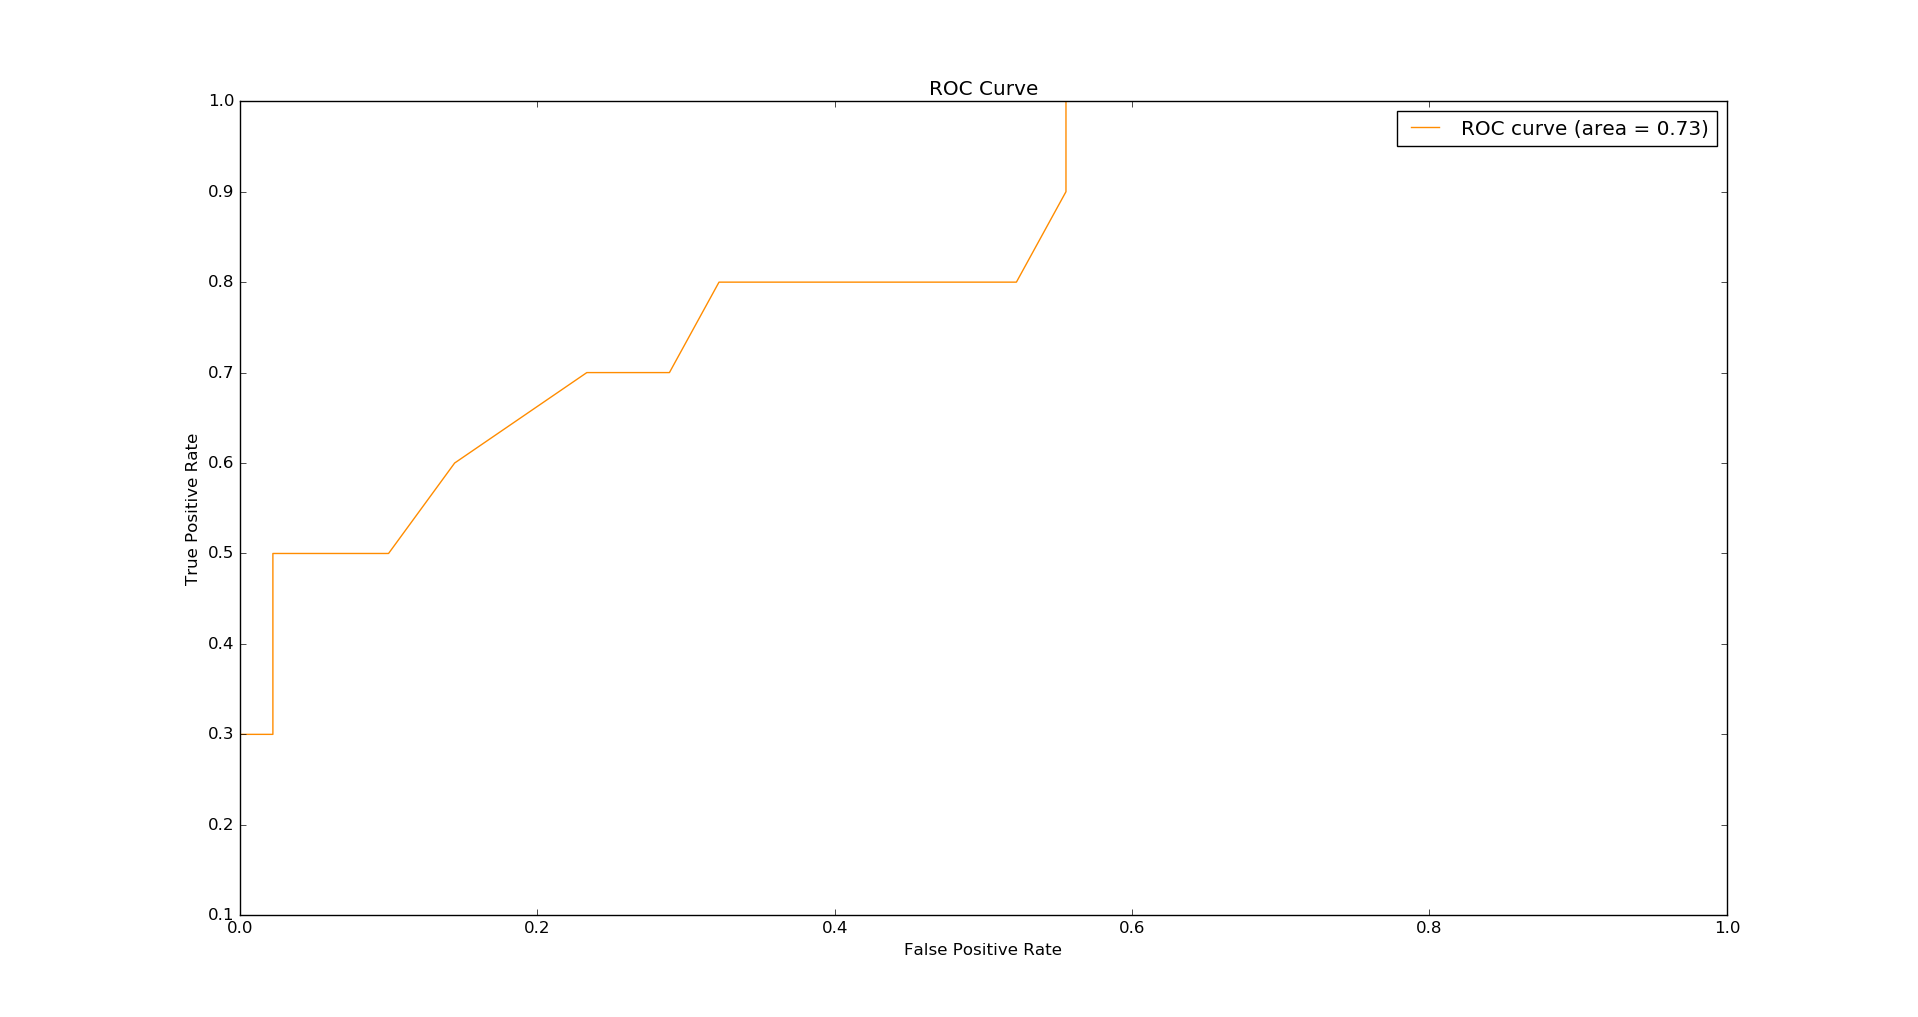
\includegraphics[width=\textwidth]{roc_auc.png}
    \caption{The ROC Curve}
    \label{fig:roc}
\end{figure}

\subsection{Threshold selection}
The goal of our classifier would be the upper left corner, where the false positive rate is 0 and the true positive rate is 1. As our classifier doesn't reach that point, we want to choose a point that is closest to this. It seems that a good value for this would be the point at false positive rate ~0.25 and true positive rate 0.7, the subpeak before the peak. The threshold there is 0.479999989271 so this would be a good value for us.
\end{document}
